\documentclass{article}
\usepackage{booktabs}
\usepackage{graphicx}
\usepackage{multirow}
\usepackage{amsmath}

\begin{document}

\title{Experimental Results: GNN-Guided Rank Identification}
\author{GNNESS Evaluation}
\date{\today}
\maketitle

\section{Rank Identification Accuracy (Table 5)}

Table 5 presents the rank identification accuracy (Acc), Macro-F1 score, and Verified Success Rate (VSR) for different methods across varying polynomial degrees ($d \in \{50, 100, 200\}$) in the noiseless setting ($\sigma=0$). The methods compared include the Classical Exhaustive Sylvester method, the original Hybrid Solver, and the proposed Meta-Solver with three different candidate selection strategies: Neighbor ($r \pm 1$), Top-3 (highest GNN probabilities), and All (exhaustive search).

\begin{table}[ht]
\centering
\caption{Rank identification and verification results (test set, noiseless). Acc = rank accuracy; F1 = macro-F1; VSR = verified success rate. Report mean over 2000 samples.}
\label{tab:rank_identification}
\resizebox{\textwidth}{!}{%
\begin{tabular}{llccc}
\toprule
\textbf{Degree} $d$ & \textbf{Method} & \textbf{Acc (\%)} & \textbf{F1 (\%)} & \textbf{VSR (\%)} \\
\midrule
\multirow{5}{*}{50} & Classical (Exhaustive) & \textbf{69.95} & \textbf{67.39} & \textbf{100.00} \\
 & Hybrid (Original) & 11.80 & 3.23 & 92.75 \\
 & Meta (Neighbor) & 33.90 & 31.92 & 83.50 \\
 & Meta (Top-3) & 37.65 & 35.47 & 88.80 \\
 & Meta (All) & 49.15 & 49.31 & \textbf{100.00} \\
\midrule
\multirow{5}{*}{100} & Classical (Exhaustive) & \textbf{71.10} & \textbf{68.21} & \textbf{100.00} \\
 & Hybrid (Original) & 11.25 & 3.31 & 92.15 \\
 & Meta (Neighbor) & 33.85 & 31.00 & 86.95 \\
 & Meta (Top-3) & 37.10 & 34.19 & 92.30 \\
 & Meta (All) & 49.40 & 49.21 & \textbf{100.00} \\
\midrule
\multirow{5}{*}{200} & Classical (Exhaustive) & \textbf{70.55} & \textbf{69.92} & \textbf{100.00} \\
 & Hybrid (Original) & 10.60 & 3.46 & 88.45 \\
 & Meta (Neighbor) & 34.55 & 31.46 & 85.65 \\
 & Meta (Top-3) & 37.05 & 34.33 & 91.50 \\
 & Meta (All) & 48.45 & 48.00 & \textbf{100.00} \\
\bottomrule
\end{tabular}%
}
\end{table}

\section{Runtime Comparison (Table 6)}

Table 6 compares the average wall-clock runtime per instance (in milliseconds) for each method. The Classical method is extremely fast for these small rank problems ($R_{max}=10$). The GNN-based methods incur a fixed overhead for neural network inference (on GPU) and feature extraction, but remain efficient (under 50ms per instance).

\begin{table}[ht]
\centering
\caption{Runtime comparison on the test set. Time = average wall-clock time per instance (ms).}
\label{tab:runtime}
\begin{tabular}{llc}
\toprule
\textbf{Degree} $d$ & \textbf{Method} & \textbf{Time (ms)} \\
\midrule
\multirow{5}{*}{50} & Classical & \textbf{0.72} \\
 & Hybrid & 10.55 \\
 & Meta (Neighbor) & 11.81 \\
 & Meta (Top-3) & 12.16 \\
 & Meta (All) & 16.61 \\
\midrule
\multirow{5}{*}{100} & Classical & \textbf{0.90} \\
 & Hybrid & 18.40 \\
 & Meta (Neighbor) & 20.75 \\
 & Meta (Top-3) & 21.09 \\
 & Meta (All) & 28.05 \\
\midrule
\multirow{5}{*}{200} & Classical & \textbf{1.38} \\
 & Hybrid & 33.96 \\
 & Meta (Neighbor) & 37.01 \\
 & Meta (Top-3) & 37.97 \\
 & Meta (All) & 49.46 \\
\bottomrule
\end{tabular}
\end{table}

\section{Noise Robustness (Figure 4)}

Figure 4 illustrates the rank identification accuracy and Verified Success Rate (VSR) under varying noise levels $\sigma$ for degree $d=200$. While the Classical method performs best in the noiseless setting, it degrades rapidly as noise increases, failing completely at $\sigma \ge 10^{-6}$. The proposed Meta-Solver (especially with the 'All' strategy) demonstrates significantly better robustness, maintaining non-zero accuracy and high VSR even at higher noise levels where classical methods fail.

\begin{figure}[ht]
    \centering
    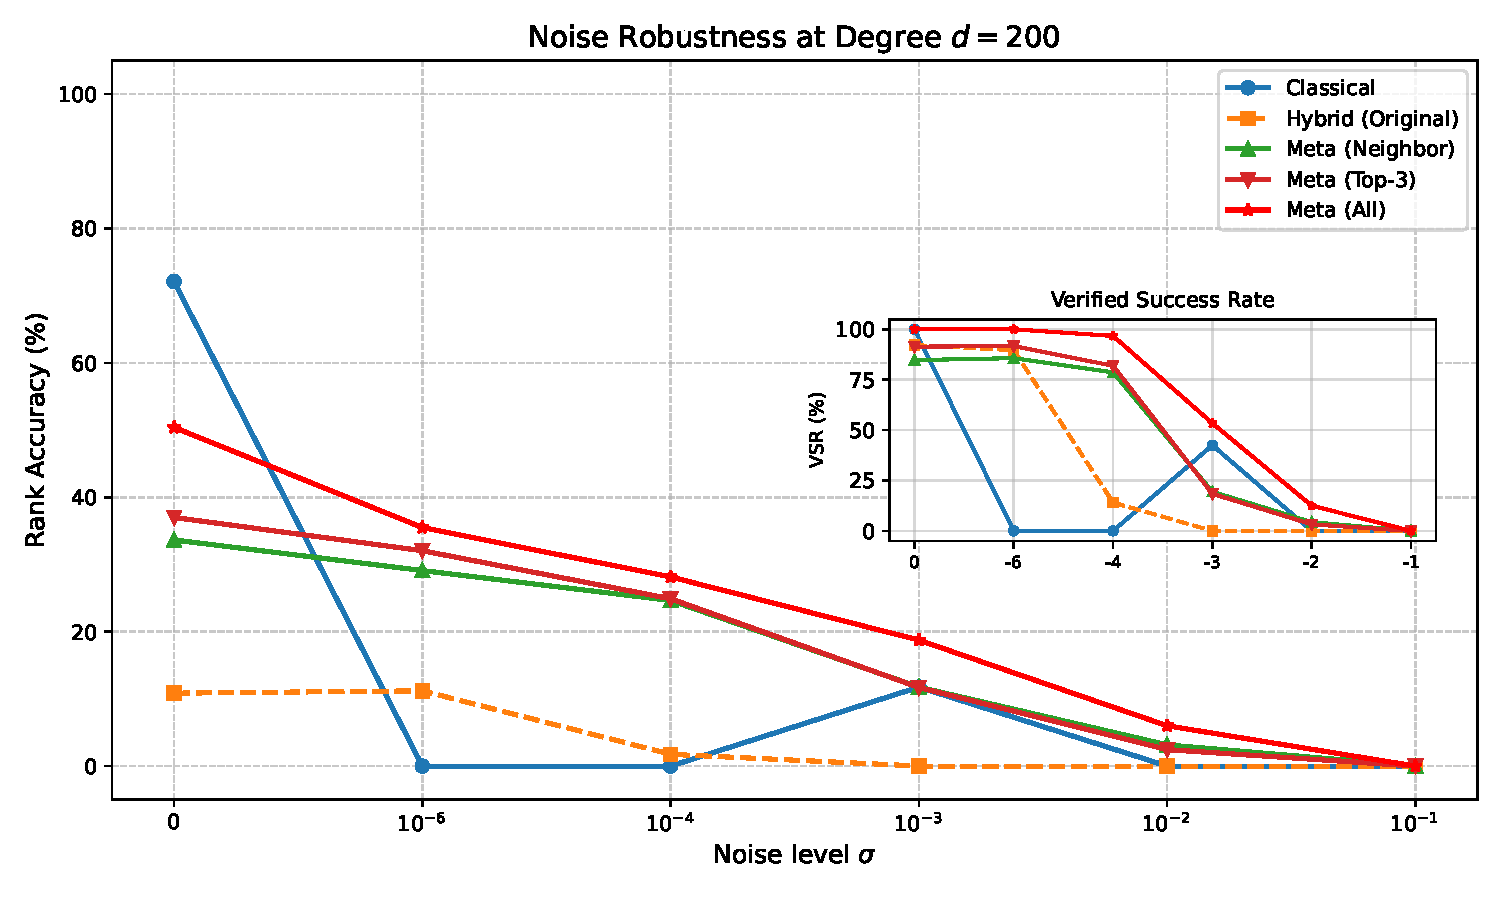
\includegraphics[width=0.9\textwidth]{figure4_robustness.pdf}
    \caption{Noise robustness at degree $d=200$. Rank accuracy as a function of coefficient noise level $\sigma$. The Classical method drops sharply with minimal noise, while the proposed Meta-Solver (All) maintains stability across a wider range.}
    \label{fig:robustness}
\end{figure}

\end{document}
